% Options for packages loaded elsewhere
\PassOptionsToPackage{unicode}{hyperref}
\PassOptionsToPackage{hyphens}{url}
%
\documentclass[
]{article}
\usepackage{amsmath,amssymb}
\usepackage{iftex}
\ifPDFTeX
  \usepackage[T1]{fontenc}
  \usepackage[utf8]{inputenc}
  \usepackage{textcomp} % provide euro and other symbols
\else % if luatex or xetex
  \usepackage{unicode-math} % this also loads fontspec
  \defaultfontfeatures{Scale=MatchLowercase}
  \defaultfontfeatures[\rmfamily]{Ligatures=TeX,Scale=1}
\fi
\usepackage{lmodern}
\ifPDFTeX\else
  % xetex/luatex font selection
\fi
% Use upquote if available, for straight quotes in verbatim environments
\IfFileExists{upquote.sty}{\usepackage{upquote}}{}
\IfFileExists{microtype.sty}{% use microtype if available
  \usepackage[]{microtype}
  \UseMicrotypeSet[protrusion]{basicmath} % disable protrusion for tt fonts
}{}
\makeatletter
\@ifundefined{KOMAClassName}{% if non-KOMA class
  \IfFileExists{parskip.sty}{%
    \usepackage{parskip}
  }{% else
    \setlength{\parindent}{0pt}
    \setlength{\parskip}{6pt plus 2pt minus 1pt}}
}{% if KOMA class
  \KOMAoptions{parskip=half}}
\makeatother
\usepackage{xcolor}
\usepackage[margin=1in]{geometry}
\usepackage{graphicx}
\makeatletter
\newsavebox\pandoc@box
\newcommand*\pandocbounded[1]{% scales image to fit in text height/width
  \sbox\pandoc@box{#1}%
  \Gscale@div\@tempa{\textheight}{\dimexpr\ht\pandoc@box+\dp\pandoc@box\relax}%
  \Gscale@div\@tempb{\linewidth}{\wd\pandoc@box}%
  \ifdim\@tempb\p@<\@tempa\p@\let\@tempa\@tempb\fi% select the smaller of both
  \ifdim\@tempa\p@<\p@\scalebox{\@tempa}{\usebox\pandoc@box}%
  \else\usebox{\pandoc@box}%
  \fi%
}
% Set default figure placement to htbp
\def\fps@figure{htbp}
\makeatother
\setlength{\emergencystretch}{3em} % prevent overfull lines
\providecommand{\tightlist}{%
  \setlength{\itemsep}{0pt}\setlength{\parskip}{0pt}}
\setcounter{secnumdepth}{-\maxdimen} % remove section numbering
\usepackage{graphicx}
\usepackage{float}
\usepackage{tikz}
\usepackage{xcolor}
\usepackage{bookmark}
\IfFileExists{xurl.sty}{\usepackage{xurl}}{} % add URL line breaks if available
\urlstyle{same}
\hypersetup{
  hidelinks,
  pdfcreator={LaTeX via pandoc}}

\author{}
\date{\vspace{-2.5em}}

\begin{document}

\section{Question}\label{question}

Los empaques sostenibles son elaborados con Cartón, Polietileno y
Aluminio, distribuidos en 6 capas, lo cual evita el contacto del
alimento con el medio externo. La gráfica muestra la distribución
porcentual aproximada de los materiales de un empaques sostenibles:

\begin{figure}[H]

{\centering 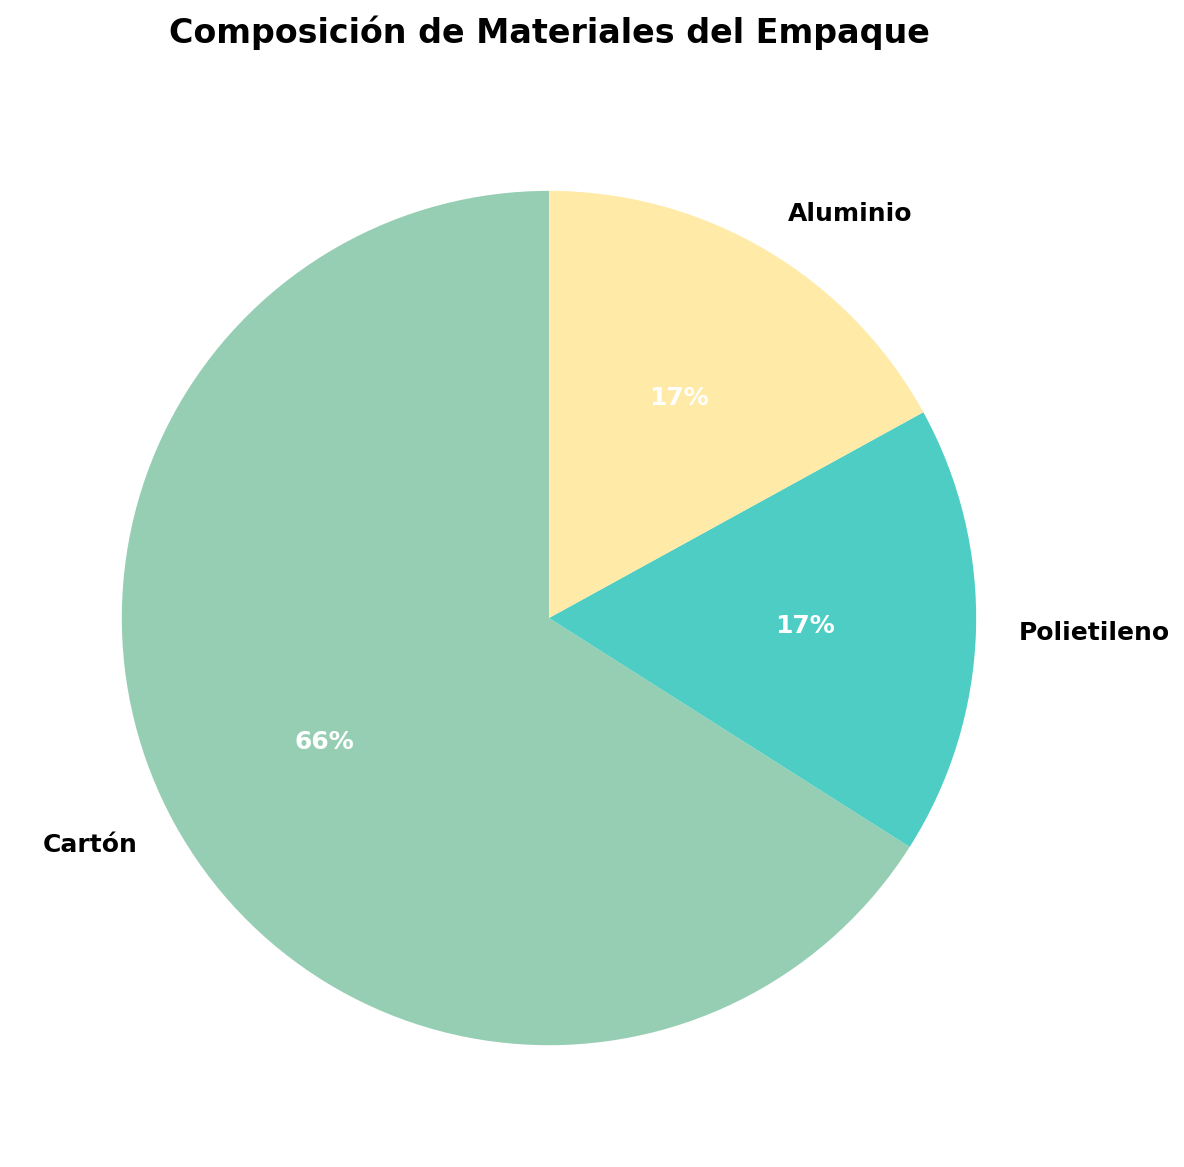
\includegraphics[width=7.53in]{grafico_composicion} 

}

\end{figure}

Las 6 capas del empaque se distribuyen así:

\textbf{Primera capa.} Polietileno: protege los alimentos de la humedad
atmosférica externa.

\textbf{Segunda capa.} Cartón: brinda resistencia, forma y estabilidad.

\textbf{Tercera capa.} Polietileno: ofrece adherencia fijando las capas
de papel y aluminio.

\textbf{Cuarta capa.} Aluminio: evita la entrada de oxígeno y luz, y la
pérdida de aromas.

\textbf{Quinta capa.} Polietileno: evita que el alimento esté en
contacto con el Aluminio.

\textbf{Sexta capa.} Polietileno: garantiza por completo la protección
del alimento.

Una persona afirma que los porcentajes de los materiales en el empaque
son válidos para un empaque de 500 ml, pero que si se construye con la
misma técnica un empaque de la mitad, reduciendo las dimensiones a la
mitad, entonces los porcentajes también se reducen a la mitad.

\textbf{Esta afirmación es falsa porque:}

\subsection{Answerlist}\label{answerlist}

\begin{itemize}
\tightlist
\item
  Los porcentajes se mantendrían porque la superficie del empaque no
  cambia proporcionalmente
\item
  Los porcentajes se conservarían sin importar el tamaño del empaque
\item
  Los porcentajes cambiarían porque el grosor de las capas no se puede
  reducir proporcionalmente
\item
  Los porcentajes se reducirían a la octava parte porque todas las caras
  se reducen a la mitad
\end{itemize}

\section{Solution}\label{solution}

Para resolver este problema de \textbf{argumentación matemática},
debemos analizar la afirmación falsa y determinar por qué es incorrecta
según los principios de escalamiento y proporcionalidad.

\textbf{Análisis de la afirmación falsa:}

La persona afirma que al reducir las dimensiones del empaque a la mitad,
los porcentajes de materiales también se reducen a la mitad. Esta
afirmación es \textbf{matemáticamente incorrecta}.

\textbf{¿Por qué es falsa la afirmación?}

\textbf{Principio fundamental:} Los porcentajes representan proporciones
relativas, no cantidades absolutas.

\textbf{Escalamiento de dimensiones:} - Factor de reducción lineal: 0,5
- Factor de reducción volumétrica: 0,5 ³ = 0,125

\textbf{Composición del empaque original:} - Cartón : 75 \% -
Polietileno : 18 \% - Aluminio : 7 \%

\textbf{Composición del empaque reducido:} Los porcentajes se mantienen
\textbf{exactamente iguales} porque:

\begin{enumerate}
\def\labelenumi{\arabic{enumi}.}
\tightlist
\item
  \textbf{Proporcionalidad:} Todos los materiales se reducen en la misma
  proporción
\item
  \textbf{Conservación de ratios:} La relación entre materiales no
  cambia
\item
  \textbf{Escalamiento uniforme:} Las 6 capas mantienen sus proporciones
  relativas
\end{enumerate}

\textbf{Demostración matemática:}

Si el empaque original tiene volumen V y el reducido tiene volumen
0,125V:

\begin{itemize}
\tightlist
\item
  Cartón original: 75\% de V
\item
  Cartón reducido: 75\% de 0,125V = 9,38\% de V
\end{itemize}

Pero como porcentaje del nuevo volumen total: 9,38\% de V ÷ 0,125V =
\textbf{75\%}

\textbf{Conclusión:}

La afirmación correcta es: \textbf{``Los porcentajes se conservarían sin
importar el tamaño del empaque''}

Los porcentajes son \textbf{invariantes bajo escalamiento uniforme}
porque representan proporciones relativas, no cantidades absolutas.

\textbf{¿Por qué las otras afirmaciones son incorrectas?}

\begin{itemize}
\tightlist
\item
  Confunden escalamiento lineal con cambios en composición
\item
  No comprenden que los porcentajes son ratios, no cantidades
\item
  Aplican incorrectamente conceptos de densidad o superficie
\item
  No reconocen la invariancia de proporciones bajo escalamiento uniforme
\end{itemize}

\subsection{Answerlist}\label{answerlist-1}

\begin{itemize}
\tightlist
\item
  Falso
\item
  Verdadero
\item
  Falso
\item
  Falso
\end{itemize}

\section{Meta-information}\label{meta-information}

exname: empaques\_tetra\_pak\_argumentacion\_escalamiento extype:
schoice exsolution: 0100 exshuffle: TRUE exsection: Argumentación en
Estadística y Proporcionalidad

\end{document}
